\chapter{Social Data in AR} % Main chapter title
\label{ch:data} % Change X to a consecutive number; for referencing this chapter elsewhere, use \ref{ChapterX}

This chapter addresses the surrounding environment of the user in terms of the social AR continuum. The surrounding environment level of detail can be determined based on the relationship between the user and the social contact with whom they are sharing the environment. The aim of this chapter is to answer the research question \ref{rq:interaction}: \textit{What is the best way to view and interact with shared social data on AR displays?}. In this chapter we study two different ways for sharing the surround environment (360 Panoramas \ref{sec:surrounding:360}, 3D scanned surroundings \ref{sec:surrounding:environment}). We also look into partially sharing/hiding \ref{sec:surrounding:hiding} part of the environment with social contacts, based on privacy concerns. For each way of sharing, we discuss the levels of detail that can be shared based on the user relationships. 

\section{Filtering Shared Social Data}
\label{sec:surrounding:360}

The social data of the surrounding scene can be described in different levels of detail. A different ways of describing a surrounding scene include: a 2D image, a panoramic image, a video, a 360-degrees video, a 3D depth image, or a VR 3D model. These different ways of describing the same scene represent the levels of details that can be varied based on the Social AR Continuum and the social proximity between the social contacts. 

This section describes a method and a prototype implementation for filtering shared social data (e.g., 360-degree videos) using wearable AR devices (e.g., HoloLens) \cite{Nassani2018a}. The data filtering is based on the sharer-viewer relationships in order to preserve privacy. For example, when sharing a 360-degrees video, if the user has an intimate relationship with the viewer, then the full fidelity (i.e., the whole 360-degree video) of the sharer's environment is visible. However, if the two are strangers, then only a snapshot image is shared, and the viewer cannot get more information about the sharer's environment. By varying the fidelity of the shared content, the viewer can focus more on the data shared by their close (in terms of social proximity) relations and differentiate this from other content. Also, this approach enables the sharer to have more control over the fidelity of the content shared with their contacts for privacy.

% In this work, we are trying to answer the question, what would be the best way to share rich data (such as 360 videos) within a large social network? The hypothesis is that filtering data based on the user-viewer relationship or proximity will increase the feeling of being together or inter-connectedness. 


% =============================================================================
\subsection{Sharing Social Data}
% =============================================================================

From the perspective of the person who is sharing the data (the sharer) with their social contacts (Figure \ref{fig:data:sharer}), the data is collected in its highest fidelity (e.g., a fully spherical 360-degree view) which will be shared with those viewers with the closest (most intimate) social relationships. For less-intimate friends, a 2D video, extracted from the 360 videos based on the sharer's view direction over time, will be shared. For Strangers, the sharer can select which snapshot image from the 2D video sequence to display. The central metaphor is that the closer the relationship that the user has to the viewer, the richer data that they can share from their point of view (360-degree videos, 2D videos, still images).

\begin{figure}[ht]
    \centering
    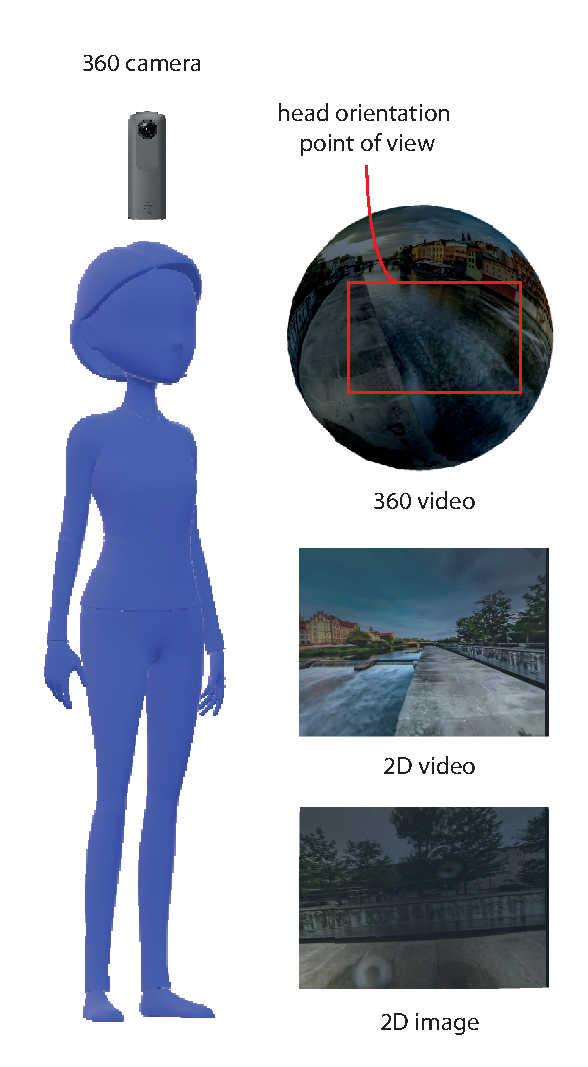
\includegraphics[width=.8\linewidth]{images/chi/images-04.eps}
    \caption{Sharing point of view with different fidelity of representation.}
    \label{fig:data:sharer}
\end{figure}

An example use-case scenario for filtering by sharer is where the sharer is going on a hike and wanting to share the experience of being in an interesting place such as near a river. The sharer takes a live 360-degree video of the surrounding environment and shares it with her followers. The sharer then gets to see how the followers are able to see the shared data based on their social relationship to her. The sharer's intimate friends and family will see the live 360-degree video, other friends the 2D video, and strangers still images of the scene, all automatically created from the 360-degree video recording.

% =============================================================================
\subsection{Viewing Shared Social Data}
% =============================================================================

The user viewing the shared data (the viewer) uses a wearable AR interface to see content from their social network superimposed over the real world, based on proxemics. For example, the viewer may be interested in seeing what their social contacts (followers) are up to and the places they have been. In this scenario the viewer can look around through the AR display to see their social contacts placed around them in three circles ordered by relationship. On top of each social contact, the viewer can see the content they are sharing, filtered based on the social relationship between the social contact and the viewer.

Based on our earlier work of representing social contacts \cite{Nassani2017a}, the people who are socially closer will appear in the AR view visually closer and have a more realistic representation. The content shared by each social contact will appear above their avatar (see Figure \ref{fig:data:viewer}), and to view the content more clearly, the user can select it (e.g., using the HoloLens air-tap gesture) to bring the content closer or walk to move inside the 360-degree video sphere. The user can then tap again to bring back the content to its original place to see other social contacts. 

\begin{figure}[ht]
    \centering
    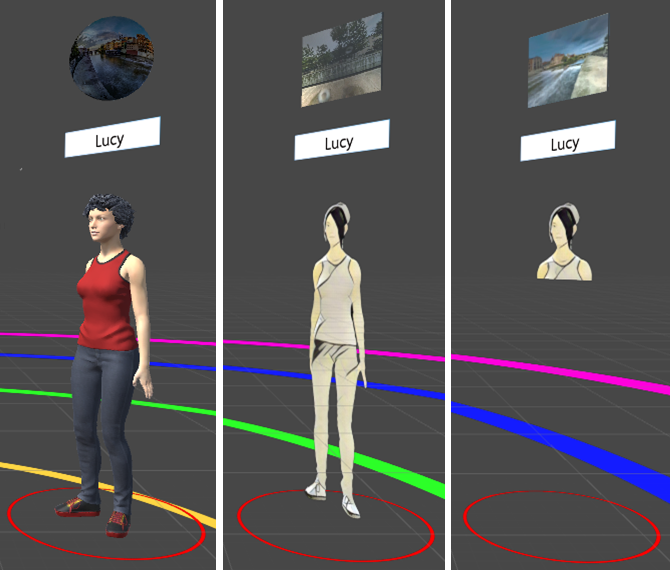
\includegraphics[width=3in]{images/chi/3_levels_of_data.png}
    \caption{Social contact sharing in different relationships with the viewer (Left to right: Intimate, Friend, Stranger). The shared data content (above the avatar) is filtered (360-degree video, 2D video, 2D image) based on social relationship.}
      \label{fig:data:viewer}
\end{figure}

In addition to this operation, this section proposes that the viewers can also see the shared content in different fidelity (360-degree videos, 2D videos or images) based on the social relationship with the sharer (Intimate, Friend or Stranger). While the sharer could restrict the fidelity of the shared content based on the social relationship as mentioned earlier, the viewer could also filter the content based on their preference. In order to avoid getting mentally overloaded by seeing too much content in high fidelity, the viewer should be able to choose the preferred fidelity for the shared content from each social contact. This could be achieved either explicitly by choosing a fidelity for each social contact, or implicitly by moving closer to or further from the avatar representing the contact.      

% =============================================================================
\subsection{Prototype}
% =============================================================================

To explore using the Social AR Continuum metaphor for sharing data between social contacts, a prototype was built using the Microsoft HoloLens. The prototype software was built using Unity 3D game engine, and it allows users to view their social contacts on a wearable AR interface. Figure \ref{fig:data:system} shows the structure of the prototype system. 

\begin{figure}[ht]
    \centering
    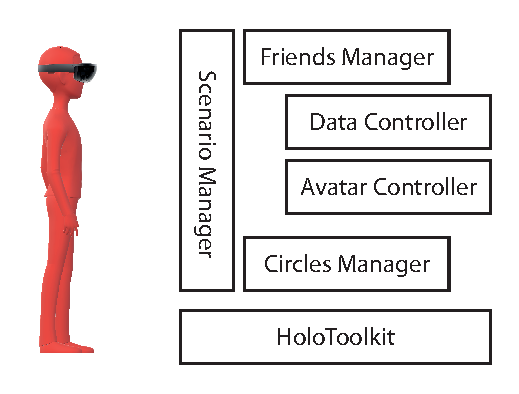
\includegraphics[width=3in]{images/chi/images-03.eps}
    \caption{System components.}
    \label{fig:data:system}
\end{figure}

The prototype places social contacts around the user (viewer) in three concentric circles which are controlled by the \textit{Circles Manager}. The social contacts have different visual fidelity and proximity based on their initial relationship to the viewer, and are rendered using the \textit{Avatar Controller}. The avatars were randomly pre-generated without any resemblance to actual contacts. MakeHuman\footnote{http://www.makehuman.org/} was used to generate the 3D avatars. The viewer (HoloLens user) can turn their head to face different social contacts and then use gestures (air taps) to interact with the contact (view their data or change their position which represents the social relationship). The interactions with HoloLens are enabled using the open-source library \textit{HoloToolkit}\footnote{https://github.com/Microsoft/MixedRealityToolkit-Unity}. The data content shared by the social contacts are controlled by the \textit{Data Controller} which determines which fidelity needs to be displayed based on the social relationship between the avatar and the viewer. The top-level \textit{Scenario Manager} defines the implementation needed for different conditions in the user study, including interaction with avatars, shared data and the concentric circles. 

% =============================================================================
\subsection{User Study}
% =============================================================================

A user study was conducted to test the system usability and effects on social presence, comparing the following conditions: 

\begin{itemize}
    \item C1) Baseline: Shows the shared 360-degree videos from all social contacts.
    \item C2) Tap-to-change: Filters the fidelity of the shared 360-degree videos based on the relationship between the viewer and the social contact. The user can tap on any social contact to cycle through different relationships.
    \item C3) Walk-to-change: Filter the fidelity of the shared 360-degree videos based on the physical distance between the viewer and the social contact.
\end{itemize}

The task was for participants to wear the headset and observe 12 social contacts (mocked up, not reflecting the participant's real social contacts) placed around the user at equal angles from each other to complete a circle (360 degrees) around the viewer, and at different distances to the viewer (centre) based on the social relationship. Each social contact had shared content floating above their head, filtered depending on the type of social relationship that the social contact had with the viewer. 

The participant could view the data content by performing the air-tap gesture on it. Once tapped, the content moved closer to the viewer. For instance, if the viewer tapped on the sphere of a 360-degree video, then the sphere immersed the participant to experience it, while for a 2D video, it was moved closer to the user so they could see it at full-screen resolution.

Participants were asked to answer the 5-point Likert-scale questions shown in Table \ref{tbl:questions} which are based on prior work \cite{Biocca2003}. Participants were asked to rate their experience on the Subjective Mental Effort Questionnaire (SMEQ) \cite{Sauro2009}. 

\begin{figure}[ht]
    \centering
    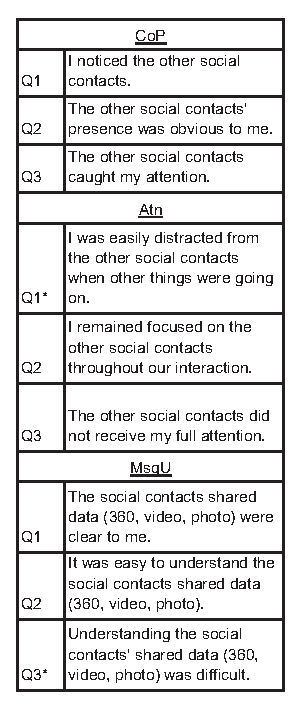
\includegraphics[width=1.5in]{images/chi/images-02.eps}
    \caption{Questionnaires for Social Presence including the following dimensions: CoPresence (CoP), Attentional Allocation (Atn), Perceived Message Understanding (MsgU). *=negative} 
      \label{tbl:questions}
\end{figure}

% =============================================================================
\subsection{Results}
% =============================================================================

A user study was run with eight participants (four female) aged 26-35 (SD=3.03). All participants used social networking platforms on a regular basis, and most (How many?) were familiar with AR/VR displays. 

After filling in a demographic questionnaire, the participants were asked to experience the three conditions in random order. Then they filled in a social presence questionnaire and SMEQ about the condition they just tried. After finishing all three conditions, participants then filled in a post-experiment questionnaire where they were asked about the overall experience and if they had any suggestions to improve it. 

From the questionnaire results (Figure \ref{fig:data:results}), indicates that C2 was rated (3.6) better in terms of social presence compared to C1 (3.3) on average, while C3 (3.5) was relatively close compared to C2. The SMEQ results show that all three conditions were rated low in terms of mental effort, while both C2 (M=16.875) and C3 (M=16.875) were rated lower than C1 (M=21).

\begin{figure}[h]
  \centering
  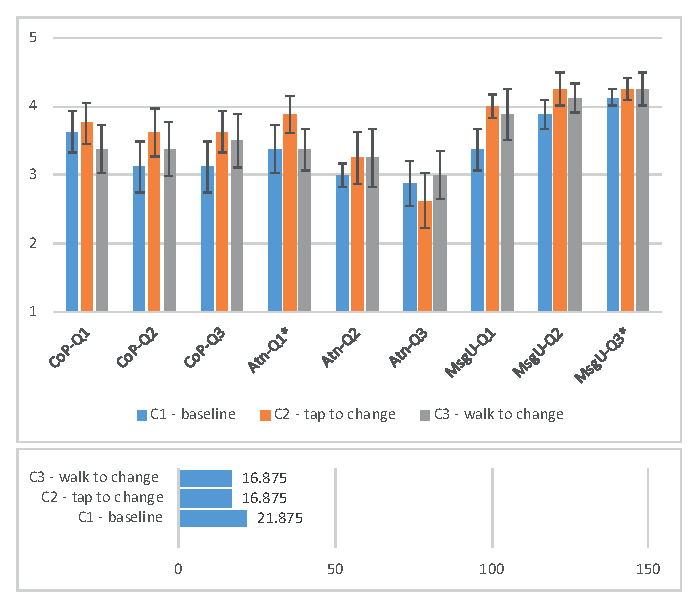
\includegraphics[width=\columnwidth]{images/chi/images-01.eps}
  \caption{Results of social presence (top) and SMEQ (bottom). *=reversed rating scale. Whiskers=standard error}
  \label{fig:data:results}
\end{figure}

As part of the post-questionnaire, participants were asked to rate the three conditions (1=least preferred, 3=most preferred). The ranking results (see Figure \ref{fig:data:ranking}) show that C1 was least preferred (1.3) while C2 (2.25) and C3 (2.375) were similar. There was a statistically significant difference in ranking conditions $\chi^2(2)=7, p=0.05$. A post-hoc analysis with Wilcoxon signed-rank tests was conducted, finding a statistically significant difference between C1-baseline and C3-Walk to change. ($Z=-2.081, p=0.037$), and no difference between the other conditions.

\begin{figure}[h]
  \centering
  
\includegraphics[width=1.5in]{images/chi/images-05.eps}
  \caption{Condition ranking results. Reverse rating scale: 1=least preferred, 3=most preferred. Whiskers=standard error. $*=$ statistically significant difference (Friedman test: $X^2(2)=7, p<0.05$).}  
      \label{fig:data:ranking}
\end{figure}

% =============================================================================
\subsection{Discussion}
% =============================================================================

From a semi-structured interview after the experiment, most users found that condition C3 (walk to change) was a more fun and natural way to view shared data from social contacts. "I feel it is more real and fun to view the 360 videos by walking toward the avatar". Also, other subjects found that the walking condition was more suitable for an outdoor or open area to avoid running into obstacles while walking. The condition C2 (tap to change) was found more convenient for changing the relationship rather than requiring more physical effort, such as walking. The Baseline condition (C1) was the least favourite for participants, as it was too overwhelming having all 360-degree videos shown all around. 

On the downside, participants mentioned some weakness for condition C2 (tap to change), such as potential clutter by being able to bring all social contacts into a small area of the intimate circle. While condition C3 (walk to change) did not have that issue, it was mentioned that by walking one might accidentally change the relationship with other social contacts that the user was not focusing on. For example, the avatars behind or on either side of the user would be affected by user movement, even if the user did not intend to get close to them. Viewing 360-degree videos through an optical see-through display was considered not as ideal, as the 360-degree videos appear to be semi-transparent on top of the real environment.

Overall, participants expressed their interest in using such a system to manage and view their social contacts and shared content in AR, and that it would be useful and easy to use. 

% =============================================================================
\subsection{Limitations and Future Work}
% =============================================================================

This prototype used asynchronous sharing, where social contacts were not online at the same time, sharing live data; the shared content was previously prepared, and the 360-degree videos were previously processed to extract 2D video and a 2D image. However, the method was applied for filtering could be applied to synchronous sharing as well. In the future, the plan is to add live video streaming from social contacts and live scaling down of the content based on social relationships. 

% The concept does apply to synchronous sharing where social contacts are online at the same time. Future plans includes extending this prototype for synchronous sharing experiences. We can expand the implementation to include spatial audio as a fidelity option on which to filter based on social relationship. 

% Additionally, we will conduct a full quantitative and qualitative user study to measure the effects of filtering content type on social presence and user experience. 

% =============================================================================
\subsection{Conclusions}
% =============================================================================

This section presented a mechanism for presenting shared data content by filtering the content type based on the social relationships between the user and the social contacts. 

This work includ an implementation on HoloLens prototype for applying the proposed method in an asynchronous collaboration scenario and conducted a user study using the prototype. The study compared three conditions: viewing 360-degree video without filtering, filtering based on the social relationship, and filtering based on distance.

Initial results showed a trend of participants favouring having the option to filter data over not filtering. The results included a qualitative feedback that provides insights for future directions. 

\pagebreak
\section{Filtering 3D Shared Surrounding Environments}
\label{sec:surrounding:environment}

As part of the Social AR Continuum for sharing social data, the previous section looked into filtering 360-degrees images and videos based on the social proximity with viewers. Sharing social data includes sharing the surrounding environment with social contacts. This section explores the social sharing of surrounding environments on wearable AR devices \cite{Nassani2018b}. In particular, it proposes filtering the level of detail of sharing the surrounding environment based on the social proximity between the viewer and the sharer. This work tests the effect of having a filter (varying the levels of detail) on the shared surrounding environment, to preserve the sense of privacy from both the viewer and the sharer perspectives, and conducted a study using the HoloLens. This section reports on semi-structured questionnaire results and suggests future directions in the social sharing of surrounding environments.

This work explores new ways of sharing the remote environment of social contacts in a wearable AR interface and builds on top of the work in the previous section \ref{sec:surrounding:360}  that looked into sharing surrounding environments based on social proximity. Previously, three levels of representing surrounding environments were tested: 360-degree video, 2d Video and 2D Image. This work focuses on sharing 3D captured rooms and levels of detail that can be used based on social proximity. 

\subsection{Prototype System}

This section describes a HoloLens prototype that was built to test different levels of detail of sharing surrounding environments. When the user puts on the HoloLens, he/she sees an AR user interface (UI) showing simulated social contacts (see Figure~\ref{fig:environment:setup}). The UI displays the social contacts around the viewer. Above each social contact avatar, the viewer can see a representation of the shared remote surrounding environment. The level of detail of the shared surrounding environment is determined by the social proximity to the viewer.

\begin{figure}
    \centering
    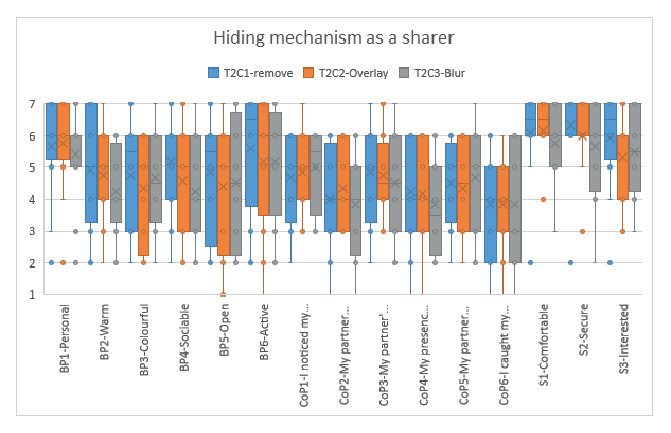
\includegraphics[width=\columnwidth]{images/53-environment-ismar18/images-06.eps}
    \caption{The viewer uses the HoloLens to view social contacts and proximity-filtered shared environments.}
    \label{fig:environment:setup}
\end{figure}

The user can air-tap on the environment above an avatar to expand it to life-size around the avatar (Figure~\ref{fig:environment:environment-levels}). The user can walk inside and explore the shared surrounding environment.

\begin{figure}
  \centering
  
\includegraphics[width=.8\linewidth]{images/53-environment-ismar18/images-05.eps}
  \caption{Levels of detail of the shared surrounding environment. 1) full details for Intimate contact: including family pictures, bank balance and computer monitor. 2) partial details for Friend contact: hiding the family picture, bank balance, but keeping work-related items such as computer monitor. 3) limited details for Stranger contact: hidden personal and work-related items.}
  \label{fig:environment:environment-levels}
\end{figure}

The prototype was built using the Microsoft HoloLens\footnote{https://www.microsoft.com/en-us/hololens} and the Mixed Reality Toolkit\footnote{https://github.com/Microsoft/MixedRealityToolkit-Unity}. The avatars representing the social contacts were generated using MakeHuman\footnote{http://www.makehumancommunity.org/}. The 3D representation of the remote sharer's room was modelled in AutoDesk Maya\footnote{https://www.autodesk.com/products/maya/overview} to simulate 3D scanning of the user's surrounding environment. 

\subsection{User Study}

The user study aimed to explore the perceived comfort as a sharer and as a viewer comparing using a filter over no filter. The study also included a semi-structured interview and asked participants about their preferred condition and hiding mechanism. To test if users preferred to have a proximity filter applied to the shared surrounding environment, the prototype offers to turn the filter on or off in two conditions: 

\begin{itemize}
    \item C1-B) no-filter (baseline)
    \item C2-F) proximity-filter (proximity filter applied)
\end{itemize}

Participants wore the HoloLens to visualise three levels of their social contacts sharing their surrounding 3D environments. Each participant tried each condition for five minutes in a counter-balanced order and answered a questionnaire after each condition. They were told to describe furniture items that are visible of their surrounding environments at each level of social relationship. At the end of the study, participants answered a few comparison questions about the preferred condition. 

\begin{itemize}
    \item Q1: As a Sharer (person sharing the surrounding environment), how do you feel about sharing the contents with others in terms of privacy? 
    \item Q2: As a Viewer (the person viewing the surrounding environment), how do you feel about sharing the contents with others in terms of privacy? 
\end{itemize}

For each condition, participants were asked to rate how comfortable they felt (on a five-point Likert scale: 1=not very comfortable, 5=very comfortable) about the sharing environment from the perspective of a sharer (person sharing) and the viewer (the person viewing) of the surrounding environment. Participants were asked to rank which condition they preferred (and to state why) from both perspectives. Finally, participants asked about which method of hiding sensitive items in the shared environment the user preferred by selecting an option from 1) remove/hide the item as if it did not exist, 2) block/overlay a black box on the item so it will be hidden, 3) blur out the item, 4) other. 

\subsection{Result}

Feedback was collected from 10 participants (five female) with an average age of 28.8 ($SD=3.65$). The participants tried demonstrations of the two conditions: C1-B (no filter), where all social contacts are sharing the full view of their surrounding environments, and C2-F (proximity filter), where the shared surrounding environments are filtered based on three levels of social proximity (Intimate, Friend and Stranger) mapped to the level of detail of the shared surrounding environment (Full, Partial and Limited). The order of the conditions was randomised based on a Latin square. 

A Wilcoxon signed-rank test was run on the subjectively perceived comfort in terms of privacy (Figure \ref{fig:environment:results}). The test showed that having a proximity filter (C2-F) applied on the shared surrounding environment did elicit a statistically significant improvement in perceived comfort in terms of privacy for both sharers ($Z=-2.831$, $p=0.005$) and viewers ($Z=-2.588$, $p=0.01$). 

As for the ranking results, C2-F (proximity filter) was preferred by both sharers (100\%) and viewers (70\%) over C1-B (no filter). C1-B (no filter) was ranked 30\% for viewers. In terms of the preferred way of hiding sensitive items in the shared environment, blurring sensitive items (60\%) was preferred followed by removing/hiding sensitive items as if they did not exist (40\%) and the lowest was overlay (10\%). 

\begin{figure}[ht]
  \centering
  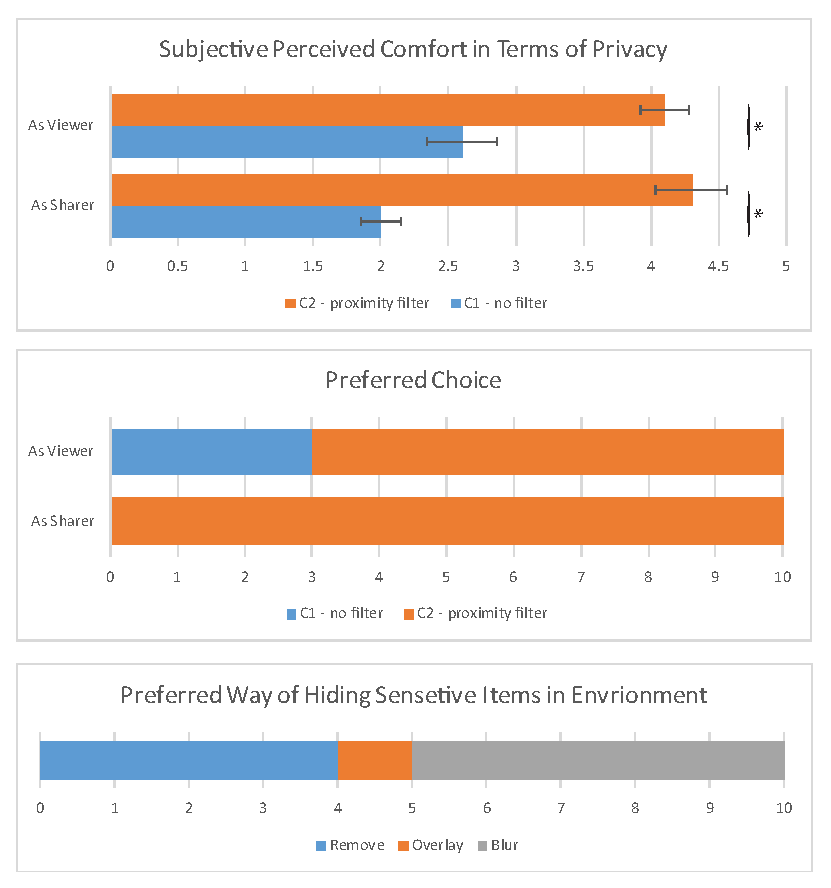
\includegraphics[width=.8\linewidth]{images/53-environment-ismar18/images-04.eps}
  \caption{Top: the average results of subjective comfort questions. Middle: the percentage results of ranking the best condition. Bottom: the percentage results of voting for the best method to hide part of the environment. Whiskers indicate the standard error.}
  \label{fig:environment:results}
\end{figure}

\subsection{Discussion}

In the open-ended questions, C1-B (no filter) was reported stronger in terms of the curiosity for the viewer. "\textit{... would suit supervisors who are interested in knowing details about their social network}", one participant mentioned. The most-reported strength of C2-F (proximity filter) was around privacy "\textit{...as a sharer, I don't want strangers to see my room}" and the sense of being comfortable in sharing levels based on social proximity "\textit{I felt more comfortable in terms of privacy}". As for weakness, C1-B (no filter) was reported to "\textit{make the sharar feels uncomfortable as everyone can see their rooms}" while for C2-F (proximity filter) the downside is more for the viewer if interested about a stranger "\textit{Although I was curious about someone who was far away from me, I couldn't get information}".

The results of preferred choice were not surprising for viewer as more participants preferred C2-F (proximity filter) over C1-B (no filter). This indicates that having a filter allows the viewer to not clutter their view with details about distant social relationships (e.g., stranger). However, some viewers preferred having no filter which allows them to see everything about everyone in their social contacts. This behaviour can be explained by human curiosity when they are viewer, and being observed in mobile and web social network as "Facebook stacking"\footnote{https://www.urbandictionary.com/define.php?term=facebook\%20stalking}. As a sharer, all participants preferred C2-F (proximity filter) which indicates that they are interested in protecting their privacy by choosing which part of the room is shared with which social relationship.

This user study is limited to the fact that the shared room is pre-configered (in terms of what is visible and hidden) for each social relationship. The next section \ref{sec:surrounding:hiding} will look into allowing the user to choose what they wan 

Overall, the results confirm our hypothesis of the value of social proximity-based filtering for sharing the surrounding environment. An interesting observation is that the sharer perspective may be different from the viewer perspective in terms of privacy. 

% In the future, we will extend this work to explore live (synchronous) sharing with both avatars and real people. Also, we will look into the perspective of the sharer and how they can select which part of the room to share with which level of social proximity contact.

\subsection{Conclusions}

This section explored implementing the Social AR Continuum on sharing surrounding environments between social contacts as one of the dimensions on the social data category. A user study was run to test the effects of applying a filter on levels of detail on how comfortable the participants were in terms of privacy. Results found that most participants are more comfortable when the social filter was applied to their shared surrounding environment.

The next section looks into sharing the social surrounding-environments from both the sharer and the viewer perspectives. Also, it examines different mechanisms of hiding/showing part(s) of the shared surrounding environments. 
\pagebreak
\section{Hiding Mechanisms of Filtering 3D Shared Surrounding Environments}
\label{sec:surrounding:hiding}

This section describes a system and a user study for hiding and showing parts of the shared social surrounding spaces on wearable AR devices. Unlike sharing for collaborative purposes, the focus of this section is on sharing between social contacts. This work extends the previous work of the Social AR Continuum by exploring how sharing the surrounding environment can vary based on the social proximity between social contacts. This work includes building a prototype for sharing a 3D captured room on a HoloLens, which enables the user to display three levels of social relationships: Intimate, Friend and Stranger, and maps them to three levels of the surrounding environment.

Previous work studied the Social AR Continuum of sharing surrounding 3D spaces by changing the level of detail of the shared 3D space based on the social proximity between viewer and sharer and focused on the viewer perspective. This work studies both the viewer and the sharer perspectives. It also allows the sharer to select which object(s) within the shared 3D space to hide or show based on the social relationship with the viewer. 

In a user study with the prototype, this work focuses on how socially connected participants felt, as well as on how they felt knowing that they were sharing more or fewer details of their surrounding environment with their social contacts. The user study found that all participant preferred having a social filter when sharing a view of their environment over having no filter. This section discusses the research findings and outlines future directions for research in sharing social surrounding spaces on wearable AR devices. 


\subsection{Background}

It is easy to imagine that in the future it will be possible for wearable AR systems to be used to capture and share a 3D view of the user's surroundings with hundreds or thousands of followers on a social network. However, before this becomes commonplace, many exciting research questions should be addressed. For example, 1) Would a person be comfortable with sharing a view of their real space with relative strangers? 2) Which items of the shared 3D room would the sharer want to hide or show to different levels of social proximity viewers? 3) Which hiding mechanism would the sharer prefer to use?

This work aims to explore how wearable AR systems could share a user's surrounding room environment with social contacts as shared content and to measure how comfortable the sharer and the viewer would feel regarding privacy in different content filtering options. The key research question of this work is how do social proximity-based content filtering and its hiding mechanisms affect feelings of co-presence and the sense of privacy and comfort for both the sharer and the viewer. The hypothesis is that social proximity-based content filtering improves social presence, co-presence and the feeling of privacy. 

% It is easy to imagine that in the future it will be possible for wearable AR systems to be used to capture and share a 3D view of the user's surroundings with hundreds or thousands of followers on a social network. However, before this becomes commonplace, many exciting research questions should be addressed. For example, 1) Would a person be comfortable with sharing a view of their real space with relative strangers? 2) Which items of the shared 3D room would the sharer want to hide or show to different levels of social proximity viewers? 3) Which hiding mechanism would the sharer prefer to use?

% This work aims to explore how wearable AR systems could share a user's surrounding room environment with social contacts and to measure how comfortable the sharer and the viewer would feel regarding privacy in different interface options. 


Previous researchers have studied the concept of "personal space" and "social bubbles" as proxemic interactions between people in different places. Greenhalgh et al. \cite{Greenhalgh1995} developed a VR teleconferencing system allowing different types of media connections (text, audio and images) between multiple users. The system was built based on the spatial model of interaction \cite{Benford1993} which defines scalability and interactions as central components of awareness consisting of an aura (total region of interaction), nimbus (region of interest and interaction) and focus of interacting objects. Sousa et al. \cite{Sousa2016} used floor projections and hand-held devices to communicate the presence of remote people, using a gradual engagement \cite{Marquardt2012} model for remote proxemics which is based on four different distances from the user; 1) personal, 2) engaged, 3) peripheral and 4) ambient.

Jo et al. \cite{Jo2016} studied the influence of the background environment (AR vs VR) and the fidelity of the remote user's avatar representation (photo-realistic vs pre-built) on co-presence. They found that more realistic avatars had a positive impact on the feeling of co-presence between remote collaborators. Volante et al. \cite{Volante2016} also studied the effect of the visual appearance of avatars (realistic vs. stylised) on the inter-personal emotional response of participants. 

Fuchs et al. \cite{Fuchs2014} studied telepresence via a scanned 3D environment to enable social connections with people and simulated face-to-face interactions. The remote person was scanned and reconstructed live in the local environment. They forecast that 3D telepresence is going to be more accessible when technology is more capable. Similarly, several companies are building social VR experiences in which users are represented as 3D virtual avatars, for example, High Fidelity\footnote{https://highfidelity.com/}, Sansar\footnote{https://www.sansar.com/}, Itsme3D\footnote{https://www.itsme3d.com/}) and other VR shared worlds. 

In the social VR space, previous work implemented a variety of visual representations of self and others. For instance, virtual avatars have been used to share social experiences such as in Facebook Spaces\footnote{https://www.facebook.com/spaces} where users can meet in VR, take selfies and teleport to a 360-degree video. Virtual avatars for self and others are represented as a floating face and upper body rendered in a VR background. 

Although there has been considerable research into social representation in VR, there has been very little research in AR. There are some challenges with AR, such as finding the best locations to fit virtual avatars in the real world, so they do not interfere with physical objects or appear suspended in mid-air. However, a social AR application can also allow people to see their social contacts while doing other tasks, i.e., users do not have to switch to an immersive VR environment to see their social contacts.

If AR is to be used to represent contacts in social networks, there could be a large number of contacts to show. If a user has hundreds or thousands of contacts in their social network, how are these to be represented in AR? In order to answer this question, we can learn from earlier work on different ways of managing large amounts of information in AR interfaces. For example, Julier et al. showed how environmental cues such as distance, and user context could be used to filter large amounts of AR content into the most relevant information that needs to be shown\cite{Julier2002}. View management techniques can also be used to ensure that virtual objects can be easily seen in collaborative AR interfaces \cite{Hollerer2001}. Similarly, an image-based approach can be used to ensure that AR information tags do not overlap in the AR view \cite{Grasset2012}. 

% Gun Lee: The background section could be stronger. Currently, it is not clear what is the main contribution/novelty of this work compared to prior work.

\subsection{System Design and Implementation}

% An AR prototype system (Figure \ref{fig:frontier18:system}) was built to run on two Microsoft HoloLens\footnote{https://www.microsoft.com/en-us/hololens} devices that are connected to each other over WiFi. The system connects a local person (the sharer) sharing a view of their surrounding physical space to a remote person (the viewer) viewing the shared virtual room overlaid on top of their physical space.

We built an AR prototype system using the Microsoft HoloLens\footnote{https://www.microsoft.com/en-us/hololens} that connects a person (the sharer) sharing a view of their surrounding physical space to a remote person (the viewer) viewing the shared virtual room overlaid on top of their physical space. Figure \ref{fig:frontier18:system} shows the components of the system that we developed.

\begin{figure}
    \begin{center}
    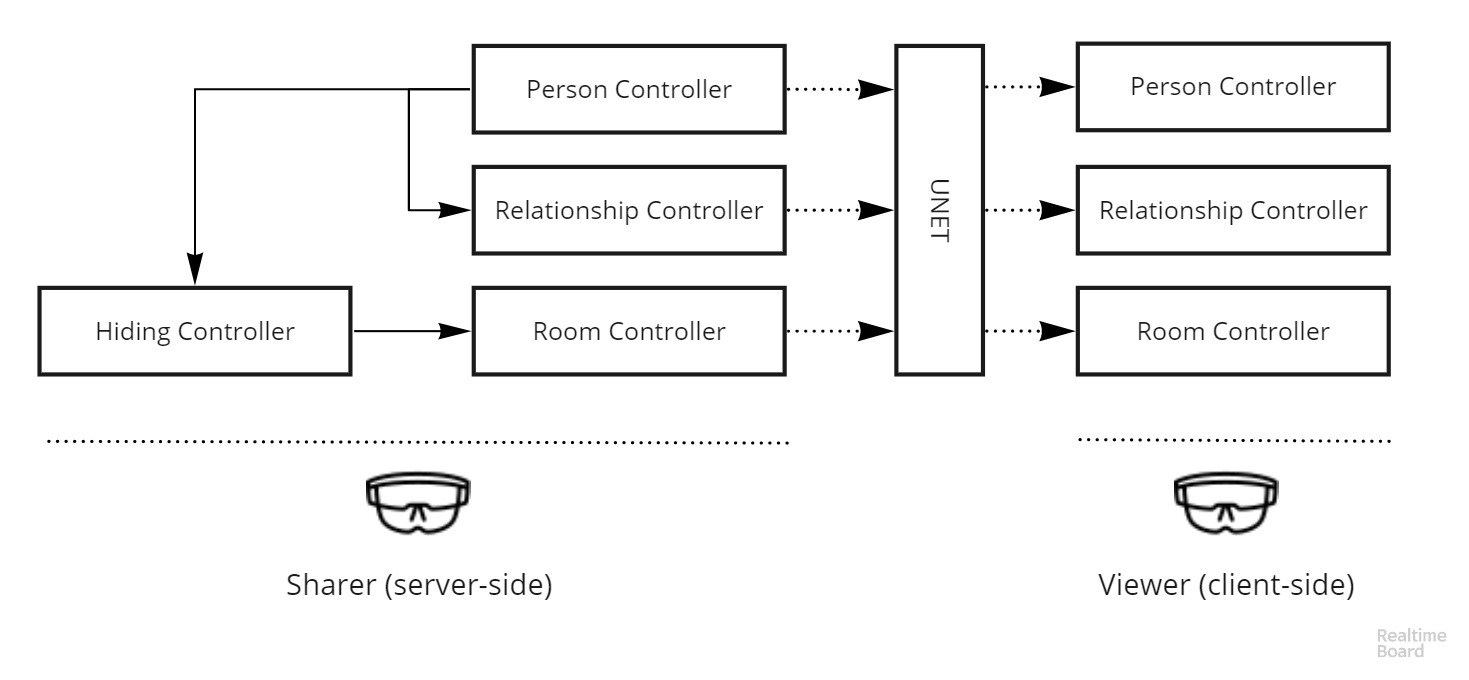
\includegraphics[width=\linewidth]{images/frontier18/system.jpg}
    \caption{System components representing the sharer server-side (left) sharing with the viewer client-side (right) via WiFi: 1) the avatar position and orientation, 2) the social relationship data and 3) room and hidden components data. The system is built on Unity and runs on a HoloLens.}
    \label{fig:frontier18:system}
    \end{center}
\end{figure}

% In the future, it will be possible to scan and immediately create a 3D model of the wearable AR user's surroundings. This was emulated by creating a virtual 3D room modelled to match the sharer's real room as if it had been 3D scanned.  The 3D modelling was done in Autodesk Maya\footnote{https://www.autodesk.com/education/free-software/maya} and rendered on the HoloLens display using the Unity3D\footnote{https://unity3d.com/} game engine. The avatars representing the remote people were generated using MakeHuman\footnote{http://www.makehumancommunity.org/}.

In the future, it will be possible for a person to scan and immediately create a 3D model of their surroundings. We emulate this by creating a virtual 3D room modelled to match the sharer's real room as if had been 3D scanned.  The 3D model of the virtual room was created on Autodesk Maya\footnote{https://www.autodesk.com/education/free-software/maya} and it was visualised on the HoloLens display using the Unity3D\footnote{https://unity3d.com/} game engine. The avatars representing the remote people (who are wearing HoloLens devices) were generated using MakeHuman\footnote{http://www.makehumancommunity.org/} and rigged to a human body using Unity3D to be animated in the AR scene. When the remote person moves in real life, the avatar moves in the same direction and orientation relative to the starting position during the experiment. 

% UNet\footnote{https://docs.unity3d.com/Manual/UNet.html} was used as the high-level networking API from Unity to synchronise the state of the shared room and the remote person. The state of the remote person includes 1) the position and orientation of the virtual avatar representing the remote person, and 2) the level of detail of the avatar based on the social relationship (i.e., Stranger=half 2D image, Friend=2D image, Intimate=3D avatar). The synchronised state of the room involves changing the level of detail of the shared room depending on the social relationship as well as which part of the room is hidden by the sharer. 

We used UNET\footnote{https://docs.unity3d.com/Manual/UNet.html}, the high-level networking API in Unity, to synchronise the state of the shared room and the remote person. The state of the remote person includes 1) the position and rotation of the virtual avatar representing the remote person, and 2) the level of detail of the avatar based on their social relationship (i.e., stranger=half 2D image, friend=2D image, intimate=3D avatar). The synchronised state of the room involved changing the level of detail of the shared room depending on the social relationship as well as which part of the room is hidden by the user. The levels of details in the shared room include 1) full room where everything is shared with the viewer, 2) partial room where most items in the room are visible, but some are hidden from the viewer, and 3) limited room where the most items are hidden, but only a few are visible to the viewer. These levels of detail of the shared room can be mapped onto three corresponding levels of social relationships (i.e., full room for an intimate relationship, partial room for friends, and limited room for strangers)

\subsection{User Study}

Using the prototype system, we wanted to investigate how filtering portions of shared environment depending on the social relationship between users affects the user's perceived the social presence and sense of privacy, and also explore various methods of filtering for maintaining privacy. To do this, we conducted a user study, with 12 participants (4 female) aged (25 - 43, median=32, SD=4.96). 
We asked participants to do two tasks: test social filter and explore hiding mechanisms for filtering.

\subsubsection{Task 1 - Social Filter}

For the first task, two participants (one sharer and one viewer) were asked to observe the shared surrounding environment (a 3D model of a room) and communicate over audio about what is visible and what is hidden in the room. The social relationship between the viewer and the sharer starts as a \textit{Stranger} relationship. The viewer then asks the sharer to upgrade the social relationship to a \textit{Friend} and then to an \textit{Intimate} relationship as a representation of a friend request on social networks. At each level of the social relationship, participants observe the changes of what is hidden and what is visible in the shared space. Two conditions are designed for this task to measure the effect of the social filter, which hides different portions and amounts of the shared surrounding space based on the social relationship. The conditions are (see Figure \ref{fig:frontier18:social-filter}): 

\begin{itemize}
\item T1C1: A shared room without a social proximity filter.
\item T1C2: A shared room with a social proximity filter. 
\end{itemize}

\begin{figure}
    \begin{center}
    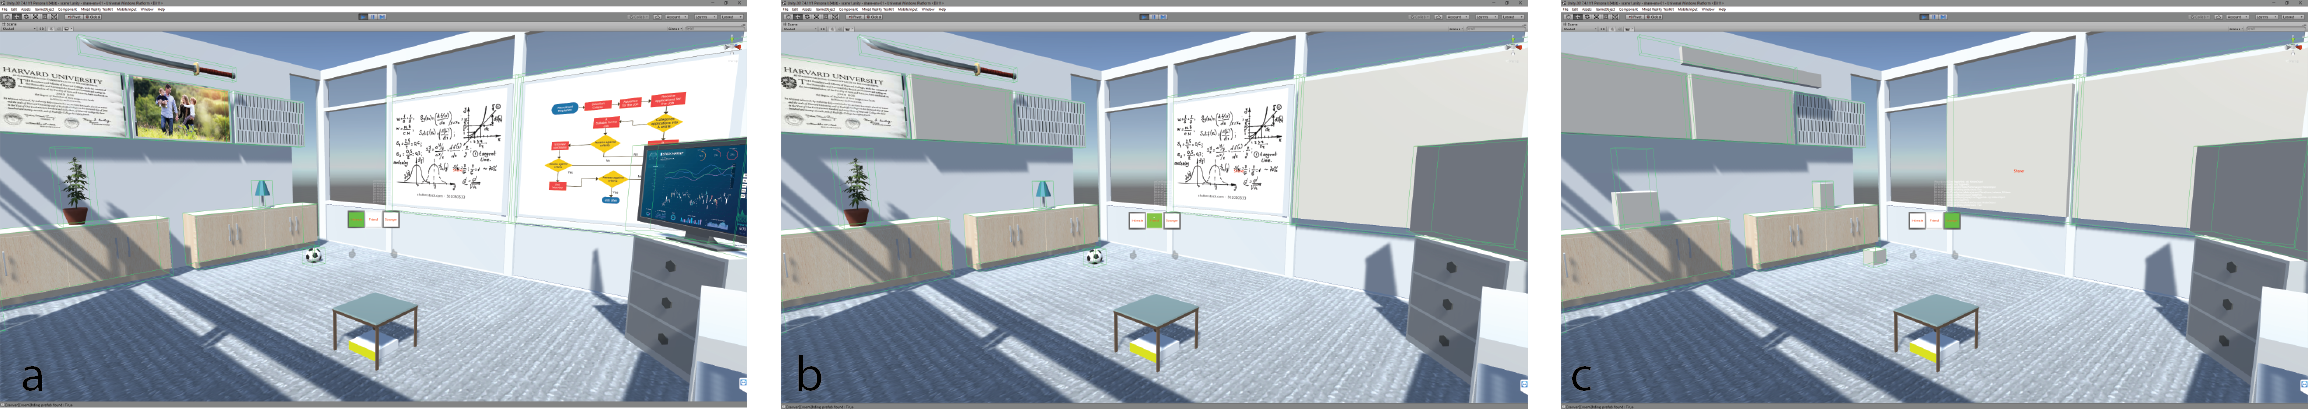
\includegraphics[width=\linewidth]{images/frontier18/images-02.png}
    \caption{A social filter applied to the shared room. a) In an Intimate relationship, everything is shared. b) For a Friend relationship, some sensitive items are hidden (e.g., family photo, stock market). c) While for a Stranger relationship almost everything is hidden in the room.}
    \label{fig:frontier18:social-filter}
    \end{center}
\end{figure}

\subsubsection{Task 2- Hiding Mechanism}

For the second task, the participants in the role of sharer were asked to select objects to hide in the shared environment. The sharer would aim at an object they wish to hide using a gaze indicator which appears at the centre of the view. The sharer would then use the air-tap gesture of the HoloLens to hide the selected object. The object is filtered out (or hidden) from the scene in one of three options: remove, overlay, and blur (see Figure \ref{fig:frontier18:hiding-mechanism}). These hiding mechanism options are the three conditions compared in this task and are described as the following:

\begin{itemize}
\item T2C1: Remove - objects are hidden by being removed from the viewer's scene.
\item T2C2: Overlay - objects are hidden by being overlaid with a virtual white box. 
\item T2C3: Blur - objects are hidden by appearing blurred to the viewer. 
\end{itemize}

\begin{figure}[h]
    \begin{center}
    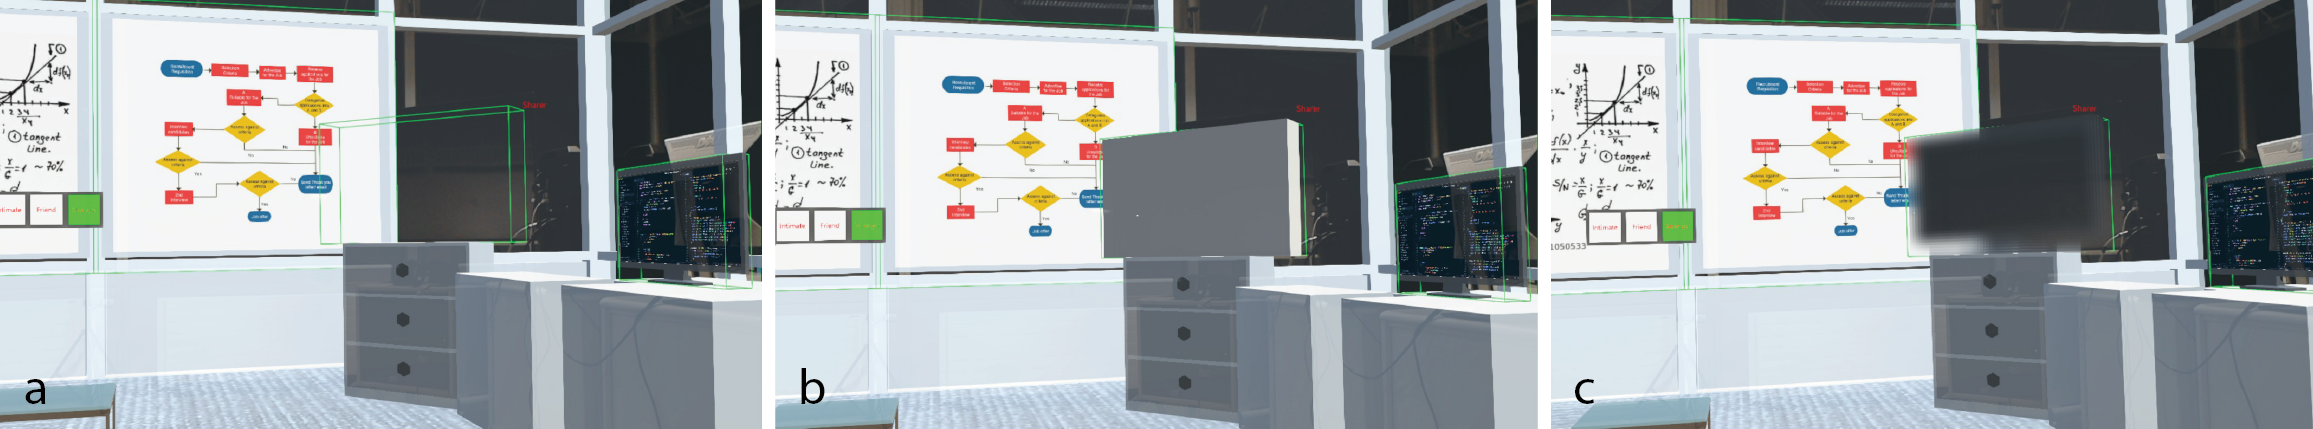
\includegraphics[width=\linewidth]{images/frontier18/images-01.png}
    \caption{Hiding mechanism applied on the TV screen. a) Remove, b) Overlay, c) Blur.}\label{fig:frontier18:hiding-mechanism}
    \end{center}
\end{figure}

% Each participant tried the conditions from both perspectives, a viewer and a sharer, in a counter-balanced order. Participants were asked to rate their experience after each condition. At the end of each task, participants were asked to compare the conditions to each other and rank them. 

% Figure \ref{fig:frontier18:setup} shows that the experiment was set up in two similar rooms so that the sharer was sharing their room with a remote viewer. The relative position and rotation of each user were synchronised and represented as a virtual avatar in the remote person view. The sharer could change the social relationship with the viewer (Intimate, Friend, Stranger) by using 3-buttons situated in the middle of the room. The viewer could request the relationship to change by clicking on one of the relationship buttons. Once this happened, the sharer saw the relationship request in a different colour, which they then could approve and change the social relationship.

The study was in a within-subject design; hence, each participant tried all of the conditions. Participating in pairs, each participant tried the conditions from both roles of being a viewer and a sharer by swapping the roles, each wearing a HoloLens device. The sharer saw their real physical environment overlaid with virtual green outline boxes for items to hide. The viewer saw the sharer's environment overlaid on top of the viewer space. Both the viewer and sharer saw each other as a virtual avatar which is positioned relative to where the users are inside the shared space. The rotation of the virtual avatar was mapped to the direction in which the users are looking. We asked participants to rate their experience after trying each condition. At the end of each task, we asked them to compare the conditions to each other and rank them. 


% Gun Lee: Not sure if this is necessary/meaningful as they are recruited in pairs, and randomly assigned to which role they are going to do first anyway.
Participants were recruited in pairs simulating a synchronous sharing experience. Participants were randomly assigned to play one of the roles (sharer or viewer) and then played the other role. The protocol of the experiment was that each participant read an information sheet and then tried a demo of the system. Each participant went through two tasks and was asked to talk to each other over an audio link about the shared surrounding environment and to notice what is shared and what is hidden in each social relationship level. 
% Gun Lee: This paragraph is redundant, as most of the study design and procedure is already described in the previous section. Better remove, or merge into the previous section?

Figure \ref{fig:frontier18:setup} shows the experiment set up in two similar rooms. The sharer was sharing his/her room with a remote viewer. The relative position and rotation of each user were synchronised and represented as a virtual avatar in the remote person's view. 
Both the viewer and the sharer were asked to explore different levels of social relationships. Both the sharer and the viewer were able to set the current social relationship using 3-buttons (intimate, friend, stranger) situated in the middle of the room. The current relationship level is highlighted using a green colour. The viewer could request the relationship to change by clicking on one of the relationship buttons. Once this happens, the sharer sees the relationship request as the button changing colour to a yellow colour, which then they could approve and change the social relationship.

\begin{figure}
    \begin{center}
    % 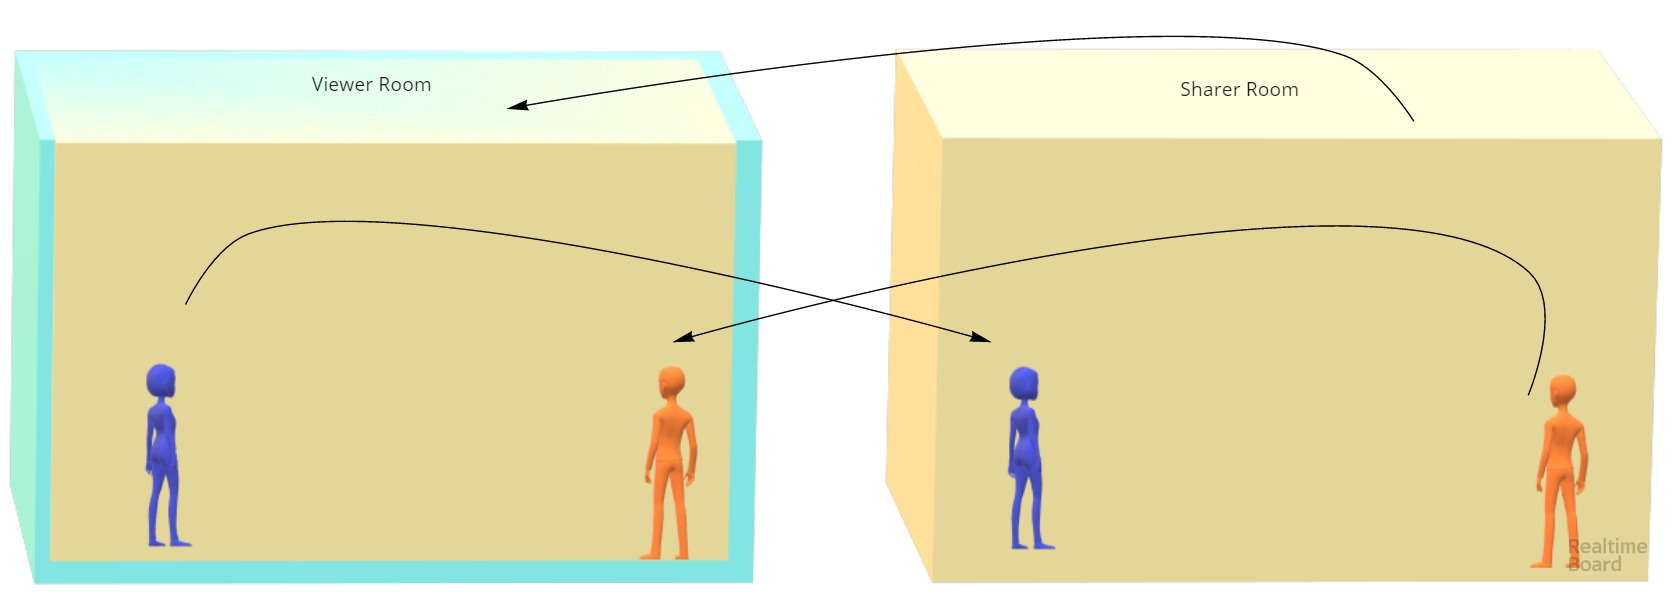
\includegraphics[width=\linewidth]{images/frontier18/experiment-setup.jpg}
    % 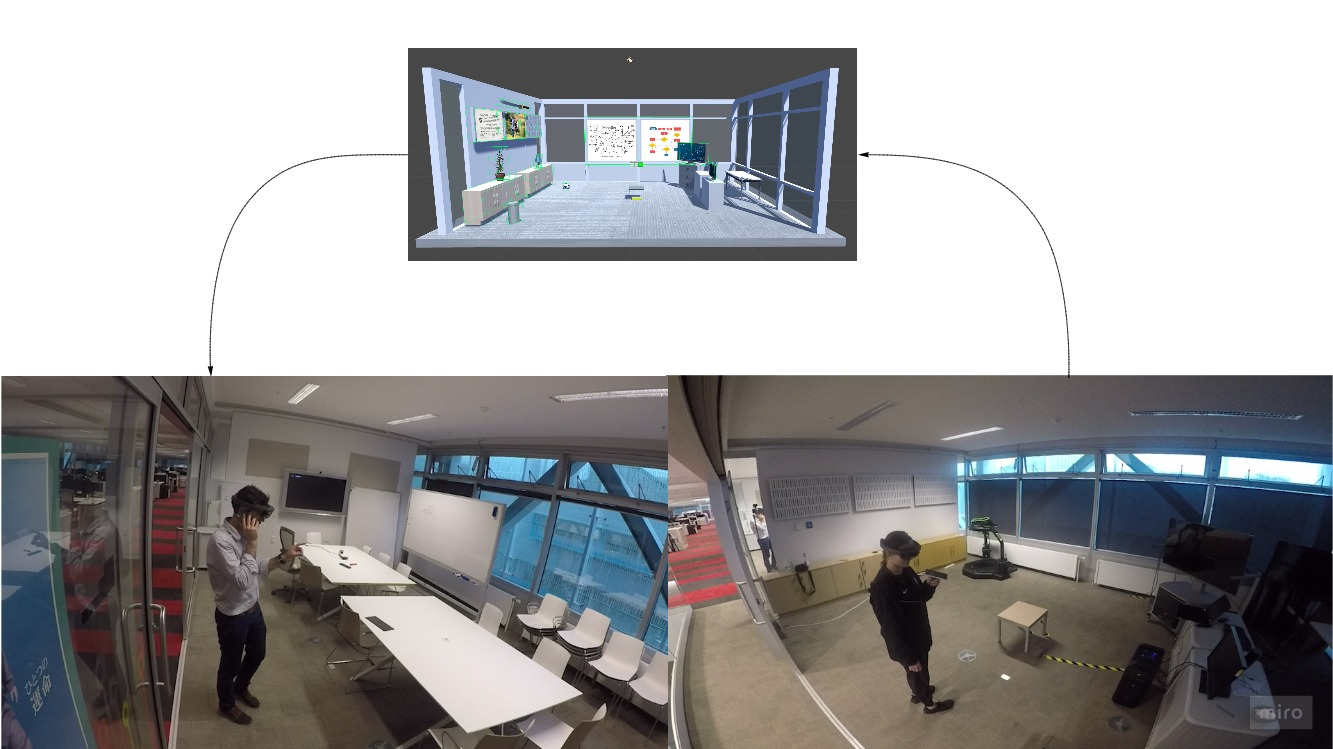
\includegraphics[width=.8\linewidth]{images/frontier18/sharing-room.jpg}
    % 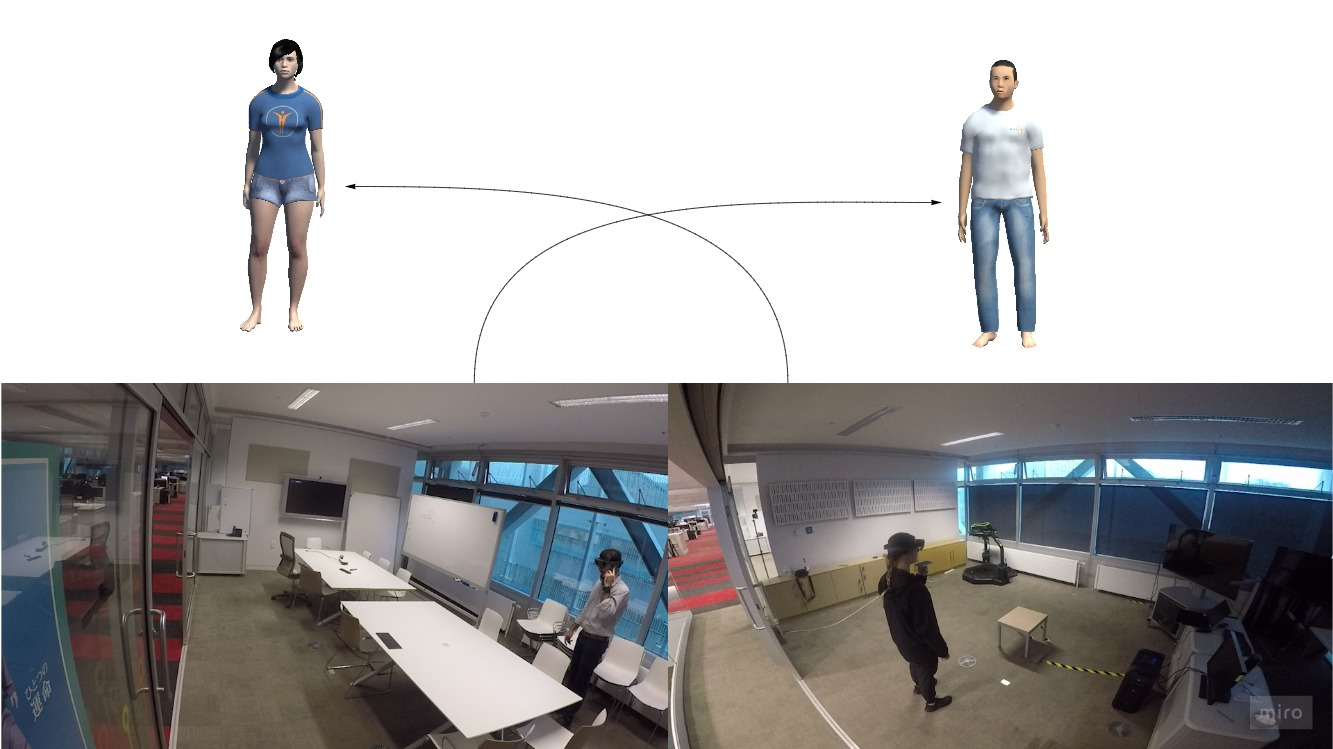
\includegraphics[width=.8\linewidth]{images/frontier18/sharing-avatar.jpg}
    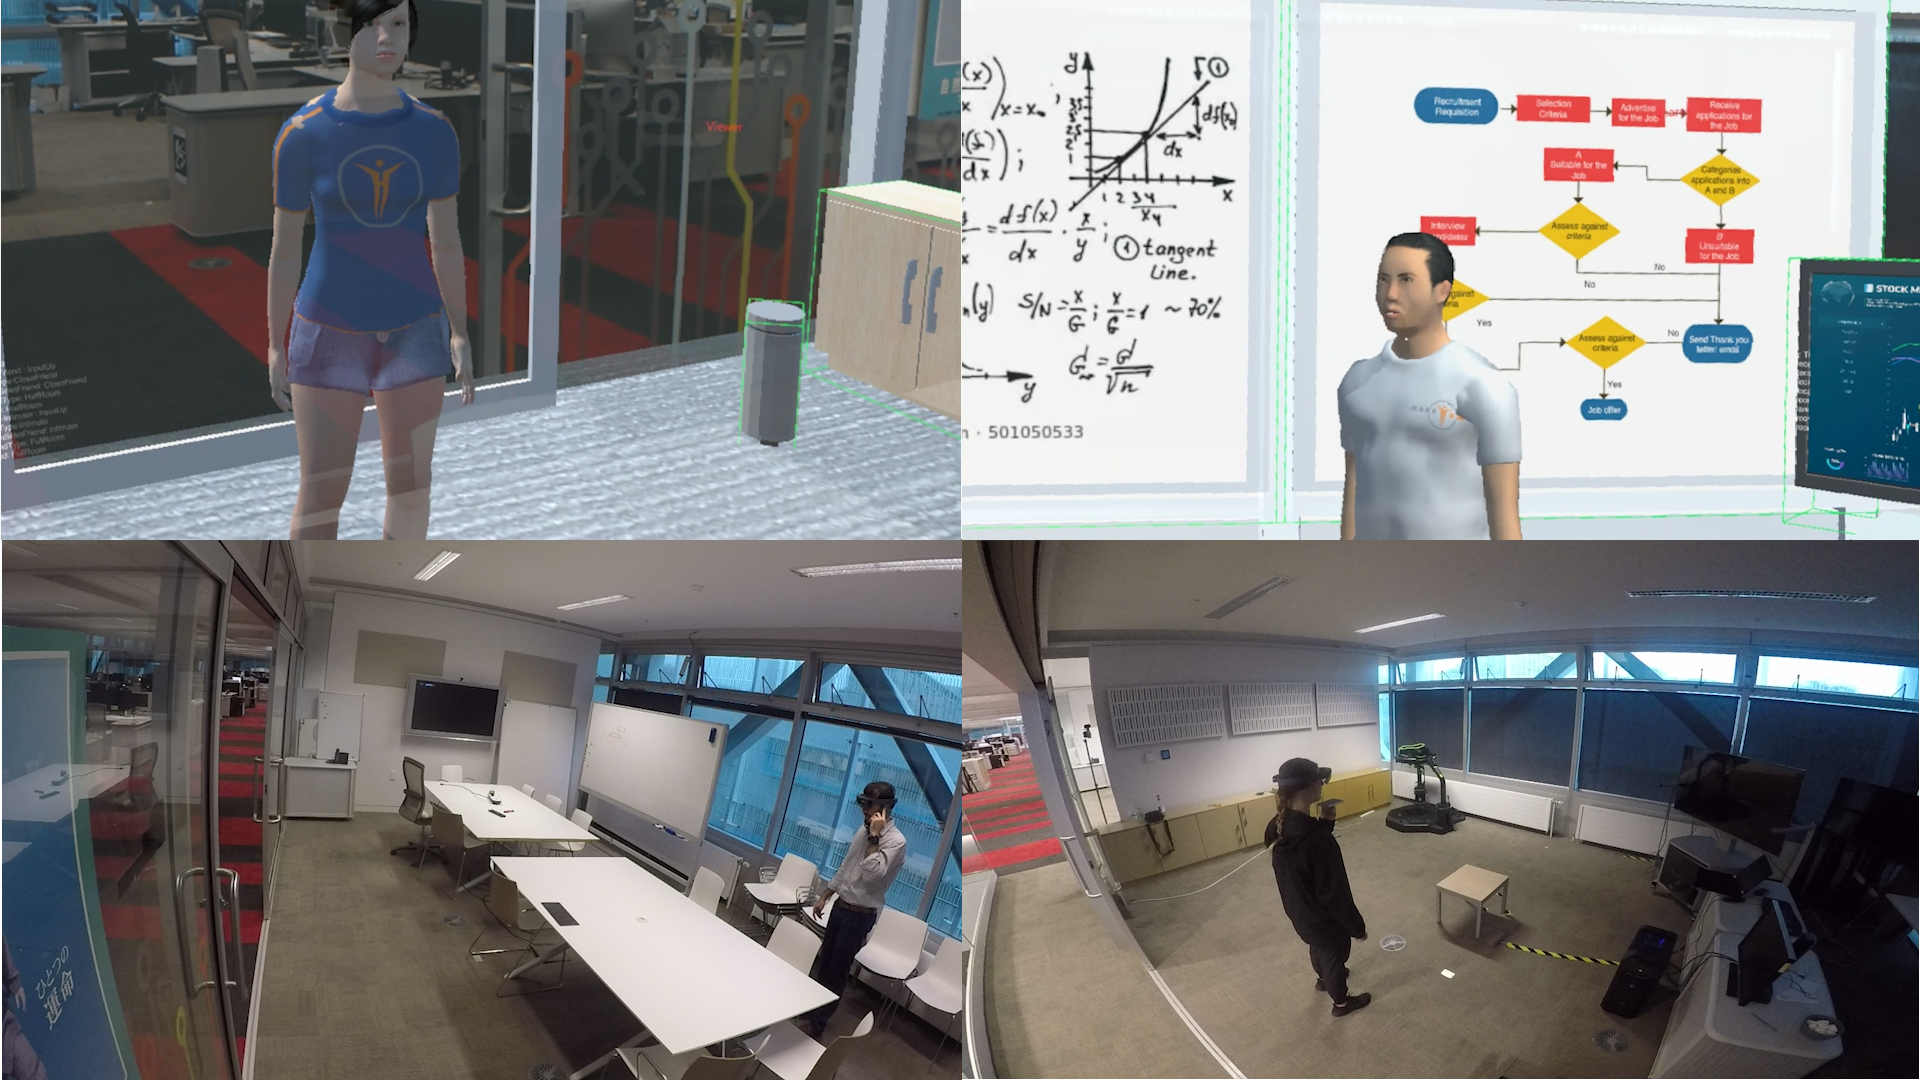
\includegraphics[width=.8\linewidth]{images/frontier18/synced.png}
    \caption{Experiment setup. The sharer (right) is sharing her room with the viewer (left). The viewer sees the virtual room of the sharer overlaid on top of his physical room. Each user sees the other person as a virtual avatar in their environment that has its position and orientation mapped to movements of the remote person.}
    \label{fig:frontier18:setup}
    \end{center}
\end{figure}

After completing each task, we asked participants to answer three sets of Likert-like questionnaires: six bi-polar questions (BP) from the semantic difference measure of social presence \cite{Smith2018}, six co-presence questions (CoP) and three shared-experience questions (S) to measure the sense of privacy (see Table \ref{tab:frontier:questions}).  

\begin{table}
    \centering
    \caption{We asked participants to rate their experience on a 7-point Likert-like scale in response to the following questions: BP=bi-polar, CoP=co-presence, S=shared-experience questions}
    \begin{tabular}{ll}
BP1 &    Impersonal-Personal\\
BP2 &    Cold-Warm\\
BP3 &    Colourless-Colourful\\
BP4 &    Unsociable-Sociable\\
BP5 &    Closed-Open\\
BP6 &    Passive-Active\\
CoP1    &   I noticed my partner\\
CoP2    &   My partner noticed me\\
CoP3    &   My partner's presence was obvious to me\\
CoP4    &   My presence was obvious to my partner\\
CoP5    &   My partner caught my attention \\
CoP6    &   I caught my partner's attention\\
S1  & Uncomfortable-Comfortable\\
S2  & Insecure-Secure\\
S3  & Not-Interested-Interested\\
    \end{tabular}
    \label{tab:frontier:questions}
\end{table}

In addition to the above rating questions, participants were asked open-ended questions about the strength and weakness of each condition. We also asked them to rank the conditions for each task from the most preferred to the least preferred condition, and then explain the reason for why they chose the best and the worst condition. 

\subsection{Results}


The summarised results shown in Figure \ref{fig:frontier18:result}. The bars indicate the mean value from all questions within the same category. The whiskers indicate standard error values. Statistically significant results are marked with *. The following subsections go into more details about the results of each question, and the statistical analysis results.

\begin{figure}
    \begin{center}
    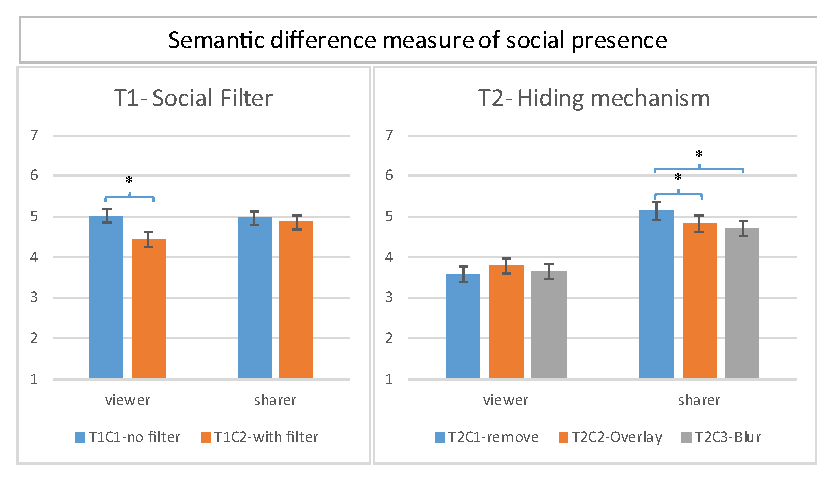
\includegraphics[width=.8\linewidth]{images/frontier18/images-17.eps}
    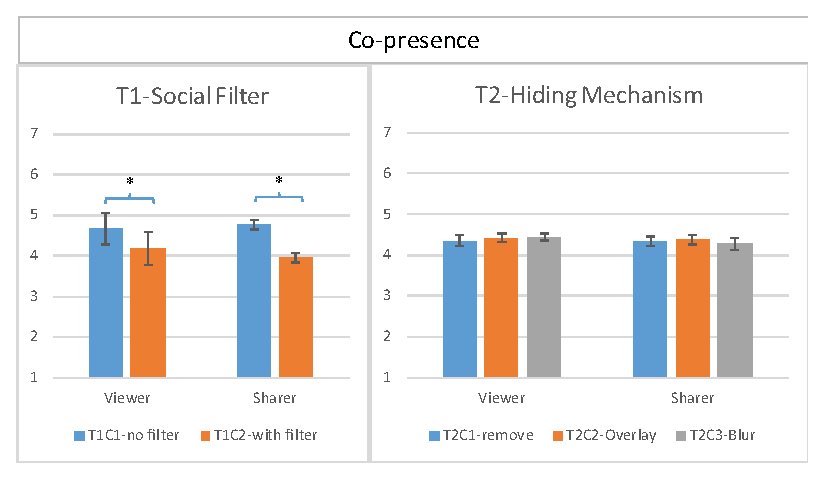
\includegraphics[width=.8\linewidth]{images/frontier18/images-16.eps}
    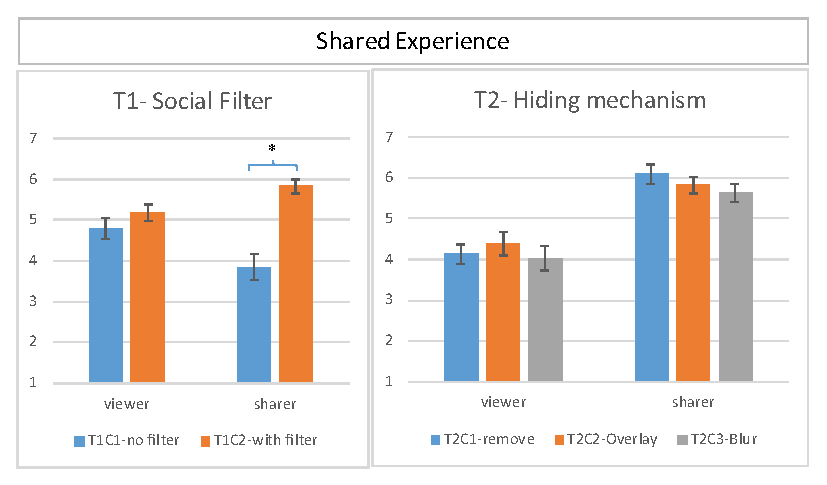
\includegraphics[width=.8\linewidth]{images/frontier18/images-18.eps}
    \caption{Results of semantic difference of Social Presence, co-presence and shared-experience questions: social filter and hiding mechanisms on a 7-point Likert scale as a viewer and as a sharer. *=statistically significant difference}
    \label{fig:frontier18:result}
    \end{center}
\end{figure}


\subsubsection{Task 1 - Social Filter}

For Task 1, Figure \ref{fig:frontier18:result-bipolar-filter} shows the Likert scale rating results for the viewer and the sharer. 
% A Wilcoxon signed-rank test on the results of \textit{Task 1} comparing no social filter (T1C1) and social filter (T1C2) showed that participants as a viewer rated significantly lower ($Z=-2.323, p=0.02$) on semantic difference bipolar rating item BP5 (Close-Open) when the social filter is applied (T1C2). However, for the sharer, there were not any statistically significant results. 

For Task 1, comparing social filter (T1C1) to social filter (T1C2), for the semantic difference measure of social presence, a Wilcoxon signed-rank test showed that T1C2 was rated statistically significantly lower ($Z=-2.843, p=0.004$) than T1C1 as a viewer. However, there was no statistical difference as a sharer ($Z=-0.421, p=0.674$).

\begin{figure}[h]
    \begin{center}
    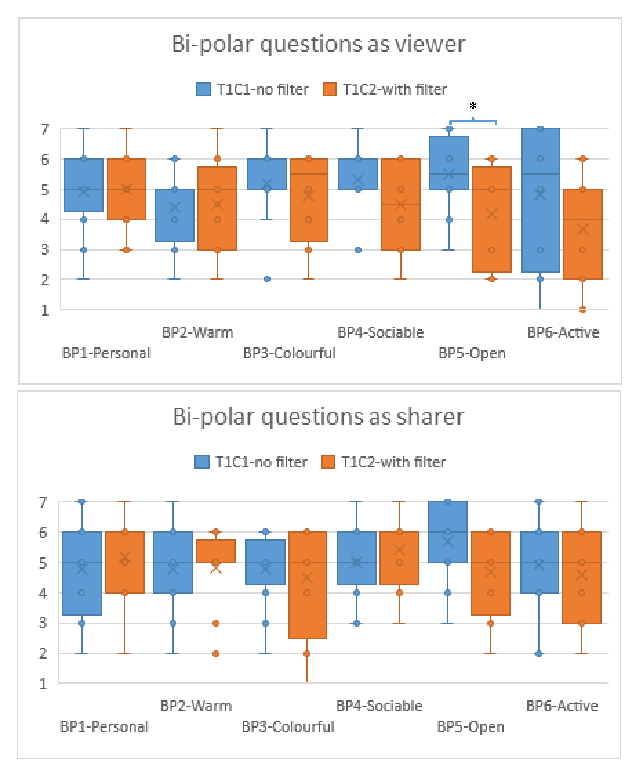
\includegraphics[width=.8\linewidth]{images/frontier18/images-13.eps}
    \caption{Average results of bi-polar questions for task 1 comparing two conditions: T1C1 no social filter to T1C2 with social filter. *=statistically significant result.}
    \label{fig:frontier18:result-bipolar-filter}
    \end{center}
\end{figure}

For the co-presence questionnaire, a Wilcoxon signed-rank test showed that T1C2 was rated statistically significantly lower ($Z=-2.444, p=0.015$) than T1C1 as a viewer and as a sharer ($Z=-3.988, p<0.000$).

% We ran a Friedman test on the co-presence questionnaire results of task 1-social filter(Figure \ref{fig:frontier18:result-copresence-filter}) and found that there was no statistically significant difference in co-presence between having a social filter (T1C2) over no social filter (T1C1) for the viewer ($X^2(2)=1.333, p=0.248$). However, there was a statistically significant difference between the results as a sharer ($X^2(2)=12.000, p=0.001$). A Wilcoxon signed-rank test showed that having a social filter did elicit a statistically significant change in co-presence as a sharer ($Z=-3.061, p=0.002$).

\begin{figure}[h]
    \begin{center}
    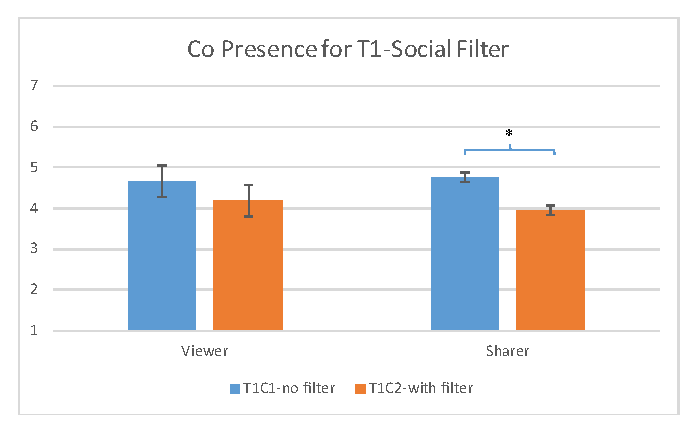
\includegraphics[width=.8\linewidth]{images/frontier18/images-10.eps}
    \caption{The average results of co-presence questions for task 1 comparing the two conditions: T1C1 no social filter to T1C2 with social filter. *=statistically significant result. Error bars indicate standard error.}
    \label{fig:frontier18:result-copresence-filter}
    \end{center}
\end{figure}


For the shared-experience questionnaire, a Wilcoxon signed-rank test showed that there was no statistical difference between T1C2 and T1C1 as a viewer ($Z=-1.689, p=0.091$); however, T1C2 was rated statistically significantly higher than T1C1 as a sharer ($Z=-4.281, p<0.000$).

% We ran a Friedman test on the shared-experience questionnaire results of task 1-social filter (Figure \ref{fig:frontier18:result-shared-experience-questions-filter}) to find that there was no statistically significant difference in shared-experience question results depending on having a social filter (T1C2) over no social filter (T1C1) as a viewer ($X^2(2)=1.000, p=0.317$). However, there was a statistically significant difference as a sharer ($X^2(2)=17.286, p<0.000$). A Wilcoxon signed-rank test showed that having a social filter did elicit a statistically significant change in co-presence as a sharer for S1-comfortable ($Z=-2.503, p=0.012$) and S2-secure ($Z=-2.816, p=0.005$), but not for S3-interested ($Z=-1.897, p=0.058$), indicating the sharers felt significantly more comfortable and secure with the social filter applied. On the other hand, participants as a viewer did not feel a significant difference between the two conditions (S1:  S2: S3: ).

\begin{figure}[h]
    \begin{center}
    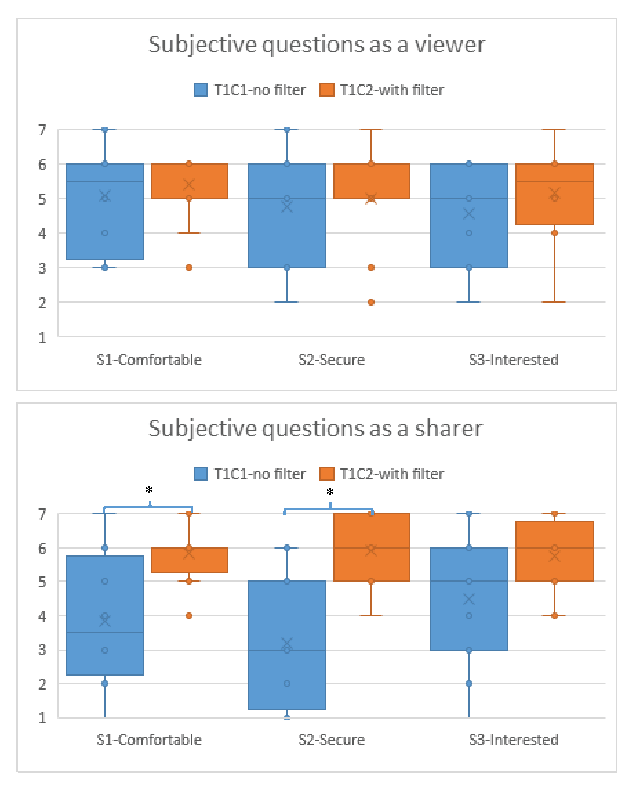
\includegraphics[width=.8\linewidth]{images/frontier18/images-14.eps}
    \caption{Results of shared-experience questions on social filter on a 7-point Likert scale as a viewer and as a sharer.}
    \label{fig:frontier18:result-shared-experience-questions-filter}
    \end{center}
\end{figure}

\subsubsection{Task 2 - Hiding Mechanism}

For Task 2, comparing hiding mechanism of 1) remove (T2C1), 2) overlay (T2C2) and 3) blur (T2C3), for the semantic difference measure of social presence, a Friedman test did not show statistically significant difference in the hiding mechanism as a viewer ($X^2(2)=3.353, p=0.187$). However, there was a statistical significance as a sharer ($X^2(2)=8.985, p=0.011$). Post-hoc analysis with Wilcoxon signed-rank test was conducted with a Bonferroni correction applied on the sharer results, resulting in a significance level set at $p<0.017$. there was a statistically significant difference between T2C1-remove and T2C2-overlay ($Z=-2.530, p=0.011$) and between T2C1-remove and T2C3-blur ($Z=-2.811, p=0.005$) but no statistical significant difference between T2C2-overlay and T2C3-blur ($Z=-1.073, p=0.283$).

% For Task 2, Figure \ref{fig:frontier18:result-bipolar-hiding} shows the Likert scale rating results for the viewer and the sharer comparing the three hiding mechanisms. A Wilcoxon signed-rank test on the results of \textit{Task 2} comparing hiding mechanism of 1) remove (T2C1), 2) overlay (T2C2) and 3) blur (T2C3) showed that as a sharer there was a statistically significant difference between blur (T2C3) and remove (T2C1) in BP4-Sociable ($Z=-2.050, p=0.040$) and CoP1-I noticed my partner ($Z=-2.000, p=0.046$). There was no difference in response to the other questions. 

\begin{figure}
    \begin{center}
    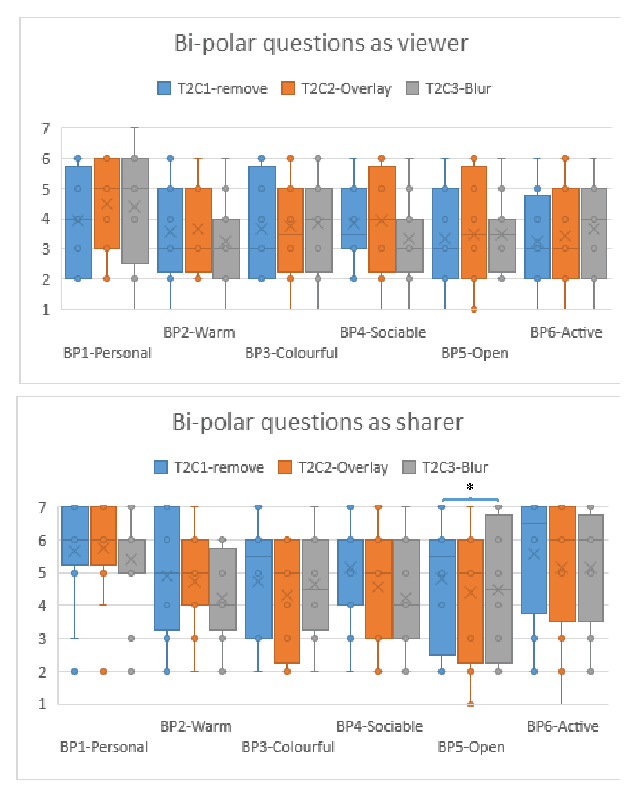
\includegraphics[width=.8\linewidth]{images/frontier18/images-12.eps}
    \caption{The average results of bi-polar questions for task 2 comparing three conditions of hiding mechanisms: T2C1-remove, T2C2-overlay and T2C3-blur. *=statistically significant result.}
    \label{fig:frontier18:result-bipolar-hiding}
    \end{center}
\end{figure}

For the co-presence questionnaire, a Friedman test did not show a statistically significant difference in the hiding mechanism as a viewer ($X^2(2)=0.419, p=0.811$) nor as a sharer ($X^2(2)=1.391, p=0.499$).

% We ran a Friedman test on the co-presence questionnaire results of task 2-hiding mechanisms (Figure \ref{fig:frontier18:result-copresence-hiding}) to find that there was no statistically significant difference in co-presence scores between the three hiding mechanisms as a viewer ($X^2(2)=0.864, p=0.649$) or as a sharer ($X^2(2)=1.217, p=0.544$).

\begin{figure}
    \begin{center}
    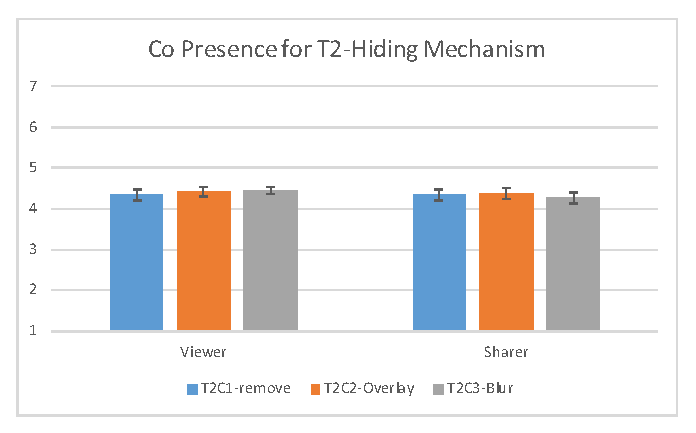
\includegraphics[width=.8\linewidth]{images/frontier18/images-11.eps}
    \caption{The average results of co-presence questions for task 2 comparing hiding mechanisms of three conditions: T2C1-remove, T2C2-overlay, T2C3-blur.}
    \label{fig:frontier18:result-copresence-hiding}
    \end{center}
\end{figure}

For the shared-experience questionnaire, a Friedman test did not show a statistically significant difference in the hiding mechanism as a viewer ($X^2(2)=3.733, p=0.155$) nor as a sharer ($X^2(2)=5.326, p=0.070$).

% We ran a Friedman test on the shared-experience questionnaire results of task 2-hiding mechanisms (Figure \ref{fig:frontier18:result-shared-experience-questions-hiding}) to find that there was no statistically significant difference in shared-experience ratings between the three hiding mechanisms as a viewer ($X^2(2)=3.733, p=0.155$) or as a sharer ($X^2(2)=5.326, p<0.070$).

\begin{figure}
    \begin{center}
    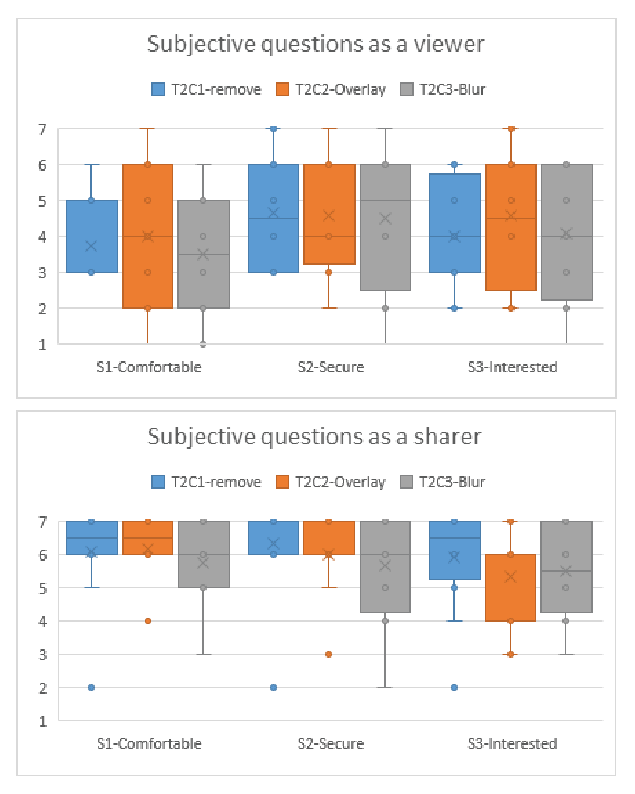
\includegraphics[width=.8\linewidth]{images/frontier18/images-15.eps}
    \caption{Results of shared-experience questions on hiding mechanisms on a 7-point Likert scale as a viewer and as a sharer.}
    \label{fig:frontier18:result-shared-experience-questions-hiding}
    \end{center}
\end{figure}

\subsubsection{Post-questionnaire}

In response to the ranking questions (Figure \ref{fig:frontier18:result-ranking}), all 12 participants preferred having a social filter when sharing a view of their room over having no filter (i.e., showing everything in the room to all social relationships). As for ranking the hiding mechanism, the most preferred option for hiding sensitive data in the room was the Remove option followed by the Overlay option, while the least preferred option was Blurring. 

\begin{figure}
    \begin{center}
    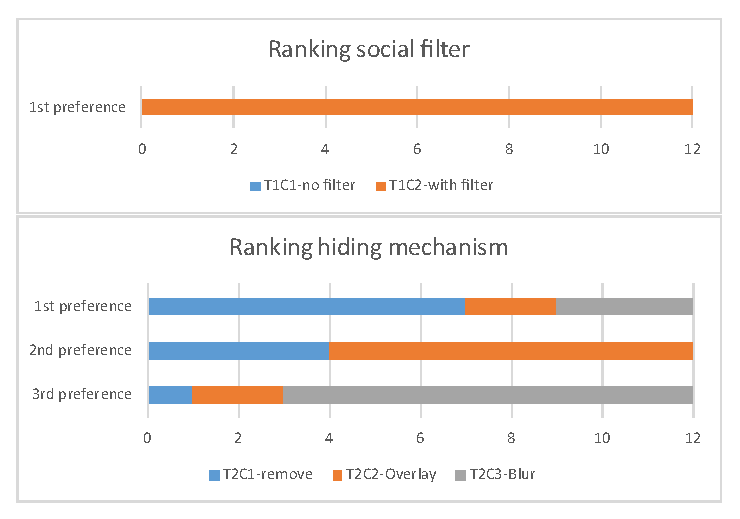
\includegraphics[width=.8\linewidth]{images/frontier18/images-19.eps}
    \caption{The results of the ranking conditions. Top: comparing no social filter to having social social filter in terms of choice preference. Bottom: comparing hiding mechanisms in terms of choice preference.}
    \label{fig:frontier18:result-ranking}
    \end{center}
\end{figure}

Participants were asked if there was a different mechanism for hiding objects in their shared room that they would prefer (such as replacing the hidden object with a similar but less sensitive one). About 42\% thought that replacing the object was a good idea; however, most of them raised concerns about how they may not like the additional effort needed for selecting a similar object to replace.

\subsection{Discussion}

For the first task of comparing using a social filter or not, the results showed a statically significant difference in the bi-polar rating item Close-Open of the semantic difference questions for the viewer side. Participants rated that they felt less Open as a viewer when having a social filter on. This can be explained by when no social filter is applied; it means nothing is hidden, and therefore, the participants may feel the sharing experience is more open. There was no statistically significant difference in the sharer side regarding semantic difference questions. 
% This indicates that from the sharer's perspective, the bi-polar questions measures are not affected by having a social filter or if no social filter is applied. 

As for the co-presence questions, there was no statistically significant difference in the viewer side whether a social filter was applied or not. This indicates that the social filter does not increase or decrease social presence for the viewer. However, from the sharer's perspective, there was a statistically significant decrease in co-presence when the social filter is applied. 
% This indicates that the sharer's feeling of co-presence is decreased when a social filter is applied. This could be because hiding part of the sharer's room with some of their social contacts reduces co-presence between the sharer and viewers. 

For the shared-experience questions, there was no statistically significant effect of having a social filter on the viewer side. However, on the sharer side, having a social filter had a significantly positive effect on users feeling comfortable and feeling secure. This indicates that having a social filter will increase the sense of being comfortable and secure for the sharer. 

For the second task of comparing hiding mechanisms, there was no statistically significant difference between the mechanisms in terms of semantic difference questions, except the bi-polar rating item Close-Open for the sharer perspective. While applying a social filter felt less open in the results of task 1, the blur hiding mechanism was rated as more open compared to the overlay and remove options. There was no statistically significant difference in co-presence and shared-experience questions. 
% This indicates that the three hiding mechanisms do not affect co-presence or the feeling of comfort, security and interest. 
% Gun Lee: repetition of the previous sentence
The ranking results showed that participants preferred having a social filter. Combined with the results of shared-experience questions, the results indicate that having a social filter is essential for people to feel comfortable regarding privacy when they have to choose, but not as much when they have to go through the effort of selecting which objects to hide for each social relationship. 
% Anthony Steed: I wouldn't rely on the number of differences as a comparator.
% Anthony Steed: Use the differences in types of difference.

\subsection{Future Work}

Future work includes allowing users to customise their room so that they feel more attached to the space they are sharing. In this user study, the sharer was hiding objects in the room while the viewer was observing the shared room at the same time. In the future, a study can be done to test if hiding before the viewer is connected would affect the sense of co-presence or the feeling of being comfortable with sharing.

% I would focus on things that extend your result.

\subsection{Conclusions}

This work described a prototype of AR social sharing experience built on a HoloLens to share a user's 3D surrounding environment with social contacts. The prototype simulates a future wearable AR social networking application. The goal of the prototype was to explore how users would be willing to share views of their surroundings with remote people with different social relationships. 

Users were allowed to choose which part of the room to hide or show to different social groups (intimate, friends, strangers). A user study was run to test the effect of using a social filter on co-presence and the feeling of privacy from both sides as a sharer and a viewer. Results showed that all participants preferred having a social filter, although it causes the feeling of being less open on the viewer side, and of lower co-presence on the sharer side. However, having a social filter had a positive effect on feeling more comfort and security on the sharer side. Results also showed that participants felt being more open when using the blur hiding mechanism compared to others, such as remove or overlay. 

\section{Summary}

This chapter explored different options of representing social data through wearable AR between social contacts. The explored options include: 1) filtering the type of shared social data, 2) filtering the level of details of shared social data, and 3) filtering partial elements in shared social data. 

The next chapter looks into the interactions between social contacts and shared social data. 
